\documentclass[format=sigconf]{acmart}
\usepackage{minted}
\usepackage{xcolor}
\usepackage{xspace}
\usepackage[utf8]{inputenc}
\usepackage[T1]{fontenc}
\usepackage{amsmath}
\usepackage{amssymb}
\usepackage{graphicx}
\usepackage{varioref}
\usepackage[nameinlink,capitalize]{cleveref}
\usepackage{tocloft}
\usepackage{amsthm} % example env
\usepackage{enumitem} % description env
\usepackage{tikz}

\usemintedstyle{xcode}
\newminted{cl}{autogobble,breaklines,escapeinside=||,fontsize=\small}

\newcommand\code[2][\small]{\sloppy\texttt{#1 #2}}
\theoremstyle{definition}
\newtheorem{example}{Example}

\usetikzlibrary{positioning,shapes,shadows}


\bibliographystyle{alpha}

\acmConference[ELS'19]{the 19th European Lisp Symposium}{April 01--02 2018}{Genova, Italy}
\acmISBN{978-2-9557474-2-1}
\acmDOI{}

\title{Implementing Baker's SUBTYPEP decision procedure}

\author{Léo Valais}
\email{lvalais@lrde.epita.fr}
\orcid{0000-0000-0000-0000}

\author{Jim E. Newton}
\email{jnewton@lrde.epita.fr}
\orcid{0000-0002-1595-8655}

\author{Didier Verna}
\email{didier@lrde.epita.fr}
\orcid{0000-0002-6315-052X}

\affiliation{%
  \institution{EPITA/LRDE}
  \streetaddress{14-16 rue Voltaire}
  \postcode{94270}
  \city{Le Kremlin-Bic{\^e}tre}
  \country{France}
}

\begin{CCSXML}
  <ccs2012>
  <concept>
  <concept_id>10011007.10011006.10011008.10011024.10011028</concept_id>
  <concept_desc>Software and its engineering~Data types and structures</concept_desc>
  <concept_significance>500</concept_significance>
  </concept>
  <concept>
  <concept_id>10003752.10003790.10011740</concept_id>
  <concept_desc>Theory of computation~Type theory</concept_desc>
  <concept_significance>500</concept_significance>
  </concept>
  <concept>
  <concept_id>10003752.10003809.10010031.10010032</concept_id>
  <concept_desc>Theory of computation~Pattern matching</concept_desc>
  <concept_significance>300</concept_significance>
  </concept>
  </ccs2012>
\end{CCSXML}

\ccsdesc[500]{Software and its engineering~Data types and structures}
\ccsdesc[500]{Theory of computation~Type theory}
\ccsdesc[300]{Theory of computation~Pattern matching}


\newcommand\sbcl{\textsc{Sbcl}}
\newcommand\then{$\rightarrow$}

\begin{document}


% \toappear{}
\begin{abstract}
  The Common Lisp standard allows the function \code{subtypep} to return
  the couple of values \code{(nil nil)} when it cannot determine the
  sub-typing relationship between two types. That permission to fail
  is granted because the type system allows the usage of the type specifier
  \code{(satisfies P)} which is understood as the type containing all the
  elements for which the predicate \code{P} return $\top$. Since \code{subtypep}
  must not evaluate \code{P}, it cannot answer many interrogations involving
  such a type specifier---hence the permission to fail. Implementations of the
  predicate often abuse such permission, making the function both inaccurate and
  unreliable. That behavior is troublesome for some applications, in particular
  for the compiler itself which uses \code{subtypep} for optimization purposes.
  Seeking for precision, H. Baker describes a decision procedure which he claims
  to be more accurate and efficient than the average implementation.
  In this article we present our partial implementation of his procedure, detail
  our understanding of his algorithm, argument in favor or against some of
  his choices and clarify parts of his description.
\end{abstract}

\maketitle

\section{Introduction}
The Common Lisp standard \cite{bib:ansi.94.cl} provides the predicate function
\code{subtypep} for
introspecting the sub-typing relationship. Every invocation \code{(subtypep A B)}
either returns the values \code{(t t)} when \code{A} is a sub-type of \code{B},
\code{(nil t)} when not or \code{(nil nil)} meaning the predicate could not
(or failed to) answer the question. The latter can happen when the type
specifier \code{(satisfies P)} (representing the type $\{x \mid
\mathtt{P(x)}\}$ for some predicate and total function\footnote{A function
  defined over its entire definition domain.} \code{P}) is involved. As shown in
\vref{lst:satisfies}, there is indeed no way for the function to answer anything
else than \code{(nil nil)} for any arbitrary predicates \code{F} and \code{G}.

However some implementations abuse of the permission to return \code{(nil nil)}.
For example, in \sbcl{} (the implementation we are currently focusing our
efforts on), {\small\code{(satisfies 'boolean 'keyword)}} returns
\code{(nil nil)}, thus violating the standard\footnote{The Common Lisp standard
  requires that no invocation of \texttt{subtypep} involving only primitive types
  returns \texttt{(nil nil)}.}. The definition of the \code{keyword} type is
responsible for the failure: as shown in \vref{lst:keyword}, it
involves a \code{satisfies} type specifier. Therefore any type-based
optimization involving determining whether \code{boolean} is a sub-type of
\code{keyword} is lost.

Another kind of problem for which \code{subtypep}'s accuracy matters is the
optimization of the \code{typecase} construct as shown in \cite{newton.18.phd}
and \cite{newton.18.els}. The aim is to remove redundant checks in the construct
and their approach is to use binary decision diagrams. However, to build such a
structure, \code{subtypep} is repeatedly used. The unreliability of the
predicate leads here to many lost BDD reductions and therefore to the
generation of not optimal code.

Our implementation is still in active development, currently targets
\sbcl{} and focuses almost entirely on results accuracy. It supports
\emph{primitive} types, \emph{user-defined} types (\code{deftype}, classes and structures),
\emph{\code{member} (and \code{eql})} type specifiers and \emph{ranges} (e.g.,
\code{(integer * 12)}). We will present our strategy for implementing each one
of these while discussing how and why we decided or not to diverge from Baker's
\cite{baker1992}
approach---or potentially filling some gaps or unclear bits.
No optimization work has been done yet and the implementation still has
bugs and diverse issues but we have found some encouraging results about
accuracy and even about efficiency.

\begin{listing}[!p]
\begin{clcode}
(subtypep '(satisfies F) '(satisfies G))
;; returns (NIL NIL)
\end{clcode}
  \caption{Impossible for \code{subtypep} to answer}
  \label{lst:satisfies}
\end{listing}

\begin{listing}
  \begin{clcode}
(sb!xc:deftype keyword ()
  '(and symbol (satisfies keywordp)))
  \end{clcode}
  \caption{The \code{keyword} type definition in \sbcl}
  \label{lst:keyword}
\end{listing}


\section{The Common Lisp type system}
\subsection{Type specifiers}
We can equivalently speak of types and sets and Common Lisp types are no
exception. They are not manipulated directly. Instead, the type to be
manipulated is \emph{described} using a \emph{type specifier}.
The type specifier DSL (Domain-Specific Language) allows the programmer to
describe types by writing S-expressions which obey some rules described in the
Common Lisp standard \cite{bib:ansi.94.cl} and roughly summarized by the
\vref{tab:ts}\footnote{More type specifiers exist. We do not describe them either
  because they are not implemented or because Baker's procedure ignores them as well.}.

A subtlety about this mechanism is that \emph{different type specifiers} can
represent the same type (e.g., \code{integer}, \code{(integer * *)} and
\code{(or fixnum bignum)} all describe the same type). It means that
\emph{symbolic computation does not suffice} to answer the sub-typing question.
As shown in \vref{lst:type=}, one could write a predicate, say \code{type=}, to
determine whether two type specifiers describe in fact the same type using
\code{subtypep}.

It is possible to define \emph{parametric aliases} using the \code{deftype}
construct. It is then possible to refer to a whole type specifier using its
alias. The \vref{lst:deftype} shows an example of \code{deftype}.

\begin{listing}
\begin{clcode}
(defun type= (type1 type2)
  (multiple-value-bind (res1 sure1-p)
      (subtypep type1 type2)
    (multiple-value-bind (res2 sure2-p)
        (subtypep type2 type1)
      (values (and res1 res2)
              (and sure1-p sure2-p)))))
\end{clcode}
\caption{The predicate \code{type=}}
\label{lst:type=}
\end{listing}

\begin{listing}
\begin{clcode}
(deftype except (x)
  `(not (eql ,x)))
\end{clcode}
\caption{The \code{deftype} construct}
\label{lst:deftype}
\end{listing}

\begin{table*}
  \centering
  \newcommand\var[1]{{\color{gray}$#1$}}
  \newcommand\pat[1]{\texttt{\small #1}}
  \begin{tabular}{rl|c}
    \hline
    Type specifier pattern & Description & Example \\
    \hline
    \pat{nil} & The null type $\emptyset$ & --- \\
    \pat{\var{t}}
            & A \code{symbol}-designated type & \code{character} \\
    \pat{(eql \var{e})}
            & The singleton type $\{e\}$ & \code{(eql 12)} \\
    \pat{(member \var{e_1} $\cdots$ \var{e_n})}
            & The type $\{e1, \cdots, e_n\}$ & \code{(member t nil)} \\
    \pat{(not \var{t})}
            & The complementary type $\overline{t}$ & \code{(not null)} \\
    \pat{(or \var{t_1} $\cdots$ \var{t_n})}
            & The union type $t_1 \cup \cdots \cup t_n$ & \code{(or integer float)} \\
    \pat{(and \var{t_1} $\cdots$ \var{t_n})}
            & The intersection type $t_1 \cap \cdots \cap t_n$ & \code{(and symbol (not keyword))} \\
    \pat{(\var{t} \var{X} \var{Y})}
            & The range $\{n \in t \mid X \leq n \leq Y\}$ & \code{(integer 1 6)} \\
    \pat{(\var{t} (\var{X}) \var{Y})}
            & The range $\{n \in t \mid X < n \leq Y\}$ & \code{(integer (0) 6)} \\
    \pat{(\var{t} * (\var{Y}))}
            & The range $\{n \in t \mid n \leq Y\}$ & \code{(integer * (43))} \\
    \pat{(array \var{t} \var{n})}
            & $n$-dimensional array of elements of type $t$ & \code{(array integer 1)} \\
    \pat{(array * (\var{d_1} $\cdots$ \var{d_n}))}
            & Array with $d_i$ elements on its $i$-th dimension & \code{(array * (3 3))} \\
    \pat{(array \var{t} (* * *))}
            & 3-dimensional $t$ array & \code{(array symbol (* * *))} \\
    \pat{(satisfies \var{p})} & The type $\{x \mid p(x)\}$ & \code{(satisfies oddp)} \\
    \hline
  \end{tabular}
  \caption{Brief summary of the type specifier DSL features}
  \label{tab:ts}
\end{table*}

\subsection{Vocabulary}
Follows some vocabulary, notations and conventions used in this article.

\begin{description}[leftmargin=8em,style=nextline]
  \item[type] For any type $t$: $t \equiv \{x \mid x\!:\!t\}$
  \item[canonical t.s.] A type specifier without aliases.
  \item[primitive type] A standardized type that is not necessarily
    implemented as a class.
  \item[symbolic form] A type specifier which type is \code{symbol}.
  \item[compound form] A type specifier which type is \code{list}.
  \item[literal type] A type specifier that only contains symbolic types,
    \code{member} types and logic compound forms.
  \item[range] A valid type specifier that consist of a single range.
  \item[interval] A mathematical interval that may not be a valid type specifier.
  \item[range type] A type specifier that only contains ranges and logic compound forms.

  \item[type $\neq$ t.s.] When no confusion is possible we take the right to
    write type specifiers where a mathematical type is expected and to use a type
    variable, say $T$, as a placeholder inside Lisp code for \emph{a type
      specifier of} $T$.
  \item[$T \subseteq T'$] The \emph{type} $T$ is a non-strict sub-type of $T'$.
    We always have \code{(subtypep $T$ $T'$)}.
  \item[$T \subset T'$] The \emph{type} $T$ is a strict sub-type of $T'$.
    We always have \code{(and (subtypep $T$ $T'$) (not (subtypep $T'$ $T$)))}.
\end{description}

\section{General procedure flow}
\vref{fig:flow} pictures the internals of our implementation. Every step will be
detailed in the following sections.

\begin{figure}
  \centering
  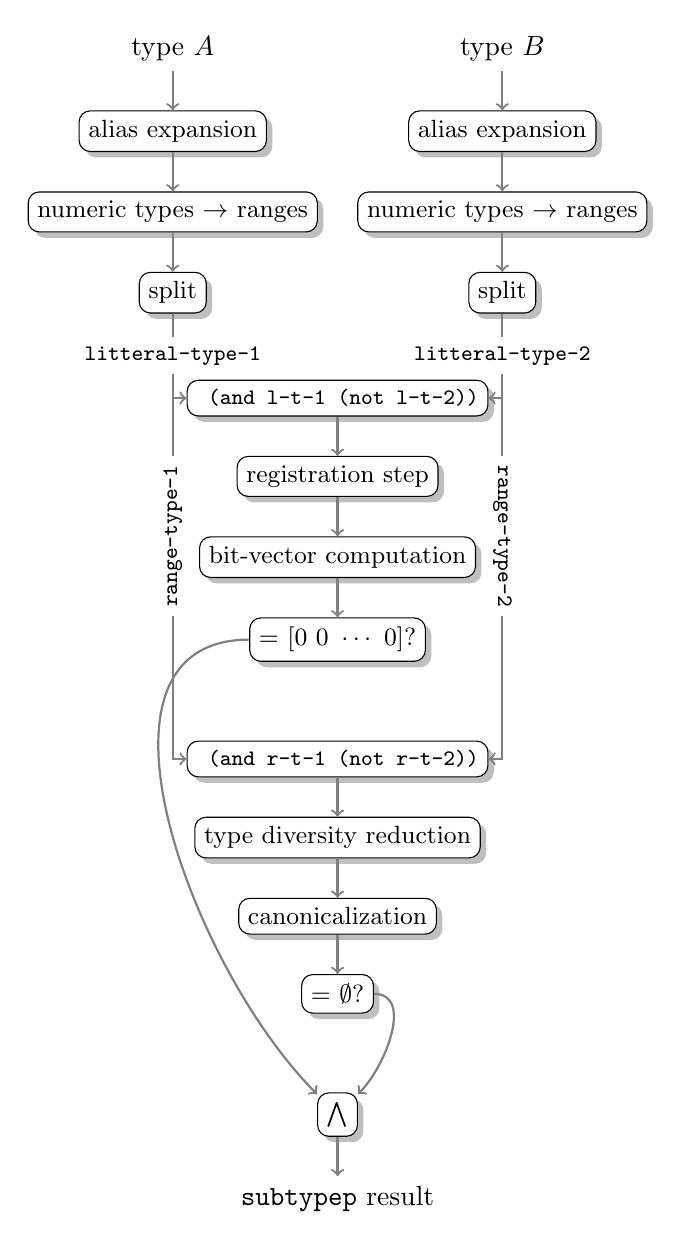
\begin{tikzpicture}[node distance=5mm,
    action/.style={rectangle,rounded corners,fill=white,drop shadow=gray,draw=black,font=\small},
    arrow/.style={->,thick,gray},
    label/.style={fill=white,text=black,font=\tt\footnotesize},
    inout/.style={}
    ]
    \def\longest{numeric types \then{} ranges}

    \node[action] (largest1) {\longest};
    \node[action,right=of largest1] (largest2) {\longest};
    \node[action,above=of largest1] (typexpand1) {alias expansion};
    \node[action,above=of largest2] (typexpand2) {alias expansion};
    \node[action,below=of largest1] (split1) {split};
    \node[action,below=of largest2] (split2) {split};
    \node[inout,above=of typexpand1] (a) {type $A$};
    \node[inout,above=of typexpand2] (b) {type $B$};
    \draw[arrow,opacity=0] (largest1) -- (largest2) node[midway,opacity=0] (middle) {};

    \node[action,below=2 of middle] (andnotL) {\code[\footnotesize]{(and l-t-1 (not l-t-2))}};
    \node[action,below=of andnotL] (reg) {registration step};
    \node[action,below=of reg] (bv) {bit-vector computation};
    \node[action,below=of bv] (nullbv) {= $[0\ 0\ \cdots\ 0]$?};

    \node[action,below=1 of nullbv] (andnotR) {\code[\footnotesize]{(and r-t-1 (not r-t-2))}};
    \node[action,below=of andnotR] (red) {type diversity reduction};
    \node[action,below=of red] (canon) {canonicalization};
    \node[action,below=of canon] (nullin) {= $\emptyset$?};

    \node[action,below=1 of nullin] (conj) {$\bigwedge$};
    \node[inout,below=of conj] (res) {\texttt{subtypep} result};


    \draw[arrow] (a) to (typexpand1);
    \draw[arrow] (b) to (typexpand2);
    \draw[arrow] (typexpand1) to (largest1);
    \draw[arrow] (typexpand2) to (largest2);
    \draw[arrow] (largest1) to (split1);
    \draw[arrow] (largest2) to (split2);

    \draw[arrow] (split1) |- (andnotR) node[label,pos=0.25,rotate=90] (rt1) {range-type-1};
    \draw[arrow] (split2) |- (andnotR) node[label,pos=0.25,rotate=-90] (rt2) {range-type-2};
    % near start = pos=0.1
    \draw[arrow] (split1) |- (andnotL) node[label,near start] (lt1) {litteral-type-1};
    \draw[arrow] (split2) |- (andnotL) node[label,near start] (lt2) {litteral-type-2};

    \draw[arrow] (andnotL) to (reg);
    \draw[arrow] (reg) to (bv);
    \draw[arrow] (bv) to (nullbv);
    \draw[arrow] (andnotR) to (red);
    \draw[arrow] (red) to (canon);
    \draw[arrow] (canon) to (nullin);

    \draw[arrow] (nullbv) to [out=180,in=135] (conj);
    \draw[arrow] (nullin) to [out=0,in=45] (conj);
    \draw[arrow] (conj) to (res);

  \end{tikzpicture}
  \caption{Internal flow for \code{(subtypep A B)}}
  \label{fig:flow}
\end{figure}

\section{Preprocessing}
% TODO add MOP bib ref for finalized classes

\section{Procedure for literal types}

\section{Conclusion and Future Work}
[..] (Flow programming @SICP)

Even if, in the future, we are to conclude that our implementation is less
efficient than those which already exists, Baker's algorithm would still likely to
improve the predicate's accuracy. Users would then have the ability to
choose whichever \code{subtypep} implementation fits their needs the best.

\bibliography{valais.19.els}

\end{document}
